% Meta-monografia de exemplo genérico de uso da classe delaetex.cls
% Copyright (C) 2004..2016 Walter Fetter Lages <fetter@ece.ufrgs.br>
%
% This file was adapted from:
% Meta-monografia de exemplo genérico de uso da classe deletex.cls
% Copyright (C) 2004 Walter Fetter Lages <w.fetter@ieee.org>
%
% This is free software, distributed under the GNU GPL; please take
% a look in `deletex.cls' to see complete information on using, copying
% and redistributing these files
%
%\documentclass[repeatfields,openright,overleaf,nomicrotype]{tcc}
\documentclass[repeatfields,xlists,xpacks,oneside,yearsonly]{ufrgscca}

\graphicspath{{./img/}}
\usepackage{fancybox}
\addbibresource{TCC.bib}

\begin{document}

\maketitle

% dedicatória é opcional
%\notoc\chapter{Dedicatória} %não vai aparecer no sumário

% agradecimentos são opcionais
%\notoc\chapter{Agradecimentos}

% Agradeço ao \LaTeX\ por não ter vírus de macro\ldots

% resumo no idioma do documento
\begin{abstract}

\end{abstract}

% resumo no outro idioma
% como parâmetro devem ser passadas as palavras-chave
% no outro idioma, separadas por vírgulas
% \begin{otherabstract}{Automation and Control, Robotics, SLAM}

% \end{otherabstract}

% sumario
\setcounter{tocdepth}{3}

% lista de ilustrações
\listoffigures

% lista de tabelas
\listoftables
% lista de listagens (código fonte)
\listofcodelist %% doesn't work on overleaf

% lista de abreviaturas e siglas
% o parametro deve ser a abreviatura mais longa
\begin{listofabbrv}{PPGEE}
    \item[ROS] Robot Operating System
    \item[BT] Behavior Tree
    \item[SLAM] Simultaneous Localization and Mapping
\end{listofabbrv}

% lista de símbolos é opcional
% \begin{listofsymbols}{$\alpha\beta\pi\omega$}
% \end{listofsymbols}

\tableofcontents

\chapter{Introdução}


\begin{figure}[htbp]
    {
        \centering
        \caption{Mercado global de robôs autônomos de 2016 a 2021, com projeção até 2028.}
        \label{fig:mercado_robo}
        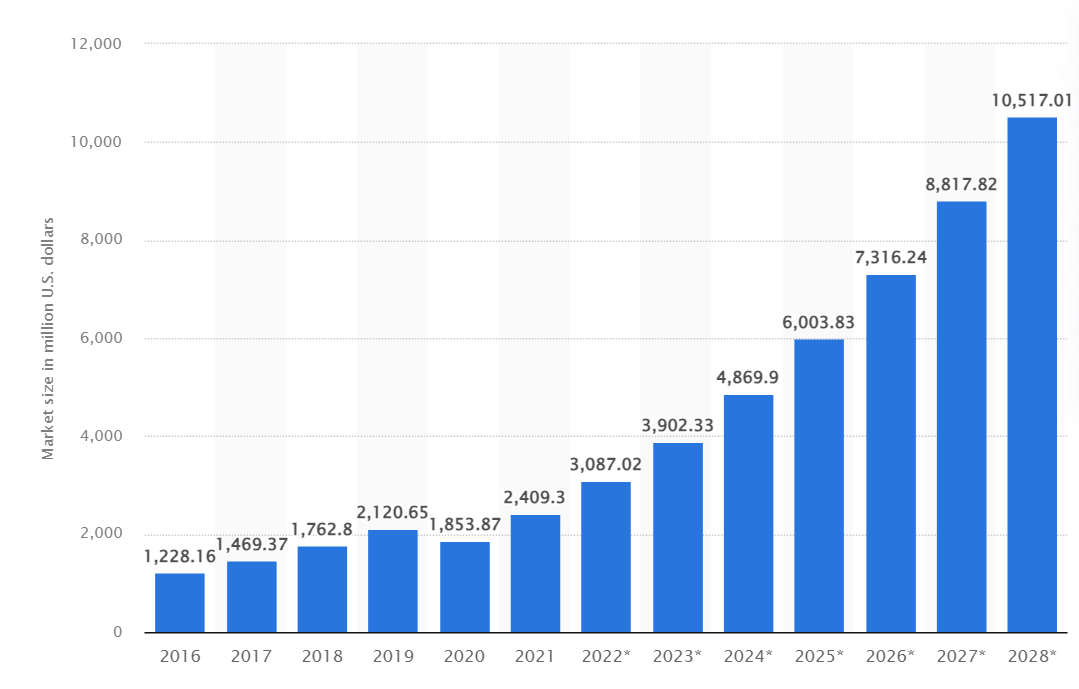
\includegraphics[width=0.8\textwidth]{mercado_robo}\\
    }
    {\sourcecitation{\textcite{robot_market}}}
\end{figure}

CITAR~\cite{amazon_robot} nome: Proteus
% Proteus autonomously moves through 
% our facilities using advanced safety,
% perception, and navigation technology developed by Amazon. 
% The robot was built to be automatically directed to perform 
% its work and move around employees—meaning it has no need to
% be confined to restricted areas. It can operate in a manner 
% that augments simple, safe interaction between technology and 
% people—opening up a broader range of possible uses to help our ...


%Robótica teve seu maior sucesso pela industria de manufatura,
%em que são utilizados manipuladores-> citar Introduction to etc
%Porém, estes robôs tem como limitação sua mobilidade.
%Um robô móvel seria capaz de se movimentar pela planta, realizando tarefas
%anteriormente não possiveis.
%O mercado para este tipo de robô está em crescimento, como mostra a
%Figura \ref{fig:mercado_robo}.
%
%Muitos desses robôs são utilizados em ambientes internos,
%como hospitais, fábricas e centros de distribuição.
%Um exemplo deste tipo de robô é o da Amazon ..
%Nestes casos, o robô está trabalhando com um ambiente dinamico e pouco conhecido,
%e por isso é necessário que o robô seja de perceber o seu ambiente e se localizar nele.
%O robô Twil, estudado neste trabalho se encaixa neste perfil, sendo um robô móvel
%
%Para solucionar novos problemas..
%Robótica é um campo novo em constante desenvolvimento\dots
%Desde os últimos trabalhos de conclusão de curso envolvendo este robô
%citar petry e rahul aqui
%houve uma grande evolução no \textit{framework} utilizado para desenvolvimento

\chapter{Revisão da Literatura}
\label{revisao}

\section{Robot Operating System(ROS2) 2}

O ROS 2 é a segunda geração do Robot Operating System,
um \textit{framework} para desenvolvimento de robôs.
Ele foi desenvolvido a partir do zero para atender as necessidades de robôs modernos,
com suporte para customização extensiva.
É baseado no padrão Data Distribution Service(DDS), que é um padrão de comunicação utilizado
em sistemas de infraestrutura crítica, como sistemas militares e financeiros~\cite{ROS2Article}.

Uma mudança relevante a este trabalho do ROS 2 é nos padrões de comunicação.
Existem três tipos de comunicação no ROS 2, \textit{topics}, \textit{services} e \textit{actions}.
\textit{Topics} são canais de comunicação unidirecionais, onde um nó publica uma mensagem
e outros nós podem se inscrever para receber essa mensagem.
\textit{Services} funcionam de forma cliente servidor, utilizando o padrão de requisição e resposta.
\textit{Topics} e \textit{services} já existiam no ROS 1.

\textit{Actions}, por outro lado, são únicos ao ROS 2.
Este padrão de comunicação é utilizado para tarefas de longa duração,
em que o cliente envia uma requisição e o servidor responde com um \textit{feedback} periódico
durante a execução, além do resultado da tarefa ao seu término, podendo ser falha ou sucesso.
Durante a execução, é possível cancelar a tarefa.

\textit{Actions} podem ser usados, por exeplo, em tarefas de navegação, em que um \textit{action client}
envia uma requisição com um ponto de destino para um \textit{action server}
que responde com um \textit{feedback} periódico da posição atual do robô e
com o resultado final.
Sua definição a torna apropriada na utilização em árvores de comportamento.

\section{Árvores de comportamento}

Árvores de comportamento, em inglês \textit{behavior trees}(BT), foram desenvolvidas
na indústria de jogos para aplicação em inteligência artificial de personagens
não jogáveis, substituindo máquinas de estado.
Elas se destacam por sua modularidade e reatividade, porém mantendo as funcionalidades
esperadas de uma máquina de estado~\cite{BehaviorTree}.

Além de seu uso na indústria de jogos, árvores de comportamento também são utilizadas
em projetos de robótica, como o robô JIBO ou
o projeto iQmatic da Scania, que utiliza árvores de comportamento no sistema de navegação
caminhões autônomos~\cite{BehaviorTree}.
Além disso, árvores de comportamento são uma peça fundamental do pacote de navegação
\textit{Navigation2} do ROS 2.

O funcionamento de uma árvore de comportamento ocorre através de uma série de
sinais enviados aos nós de uma árvore com uma frequência fixa.
Este nó responde com o estado atual da execução, que pode ser \textit{running},
se está em execução, \textit{success}, se atingiu o objetivo, ou \textit{failure}
nos demais casos.
Na formulação clássica, existem quatro categorias de nós de controle(\textit{Sequence},
\textit{Fallback}, \textit{Parallel} e \textit{Decorator}) e duas categorias
de nós de execução(\textit{Action} e \textit{Condition}).
A Tabela \ref{tab:bt_nodes} mostra os símbolos utilizados para representar
os nós de uma árvore de comportamento.

\begin{table}[htb]
    \begin{center}
        \caption{Símbolos dos nós de uma árvore de comportamento.}
        \label{tab:bt_nodes}
        \begin{tabular}{cc}
            Tipo de nó         & Símbolo                    \\                    %& Sucesso                             & Falha                                & Executando                     \\
            \hline
            \textit{Fallback}  & \fbox{?}                   \\                   %& Se um filho retorna sucesso         & Se todos filhos retornam falha       & Se um filho retorna executando \\
            \textit{Sequence}  & \fbox{$\rightarrow$}       \\       %& Se todos filhos retornam sucesso    & Se um filho retorna falha            & Se um filho retorna executando \\
            \textit{Parallel}  & \fbox{$\rightrightarrows$} \\ %& Se $\geq M$ filhos retornam sucesso & Se $ > N - M$ retornam falha         & Nos outros casos               \\
            \textit{Action}    & \fbox{texto}               \\               %& Se atinge o objetivo                & Se não é possível atingir o objetivo & Durante execução               \\
            \textit{Condition} & \ovalbox{texto}            \\            %& Se é verdade                        & Se é falso                           & Nunca                          \\
            \textit{Decorator} & $\Diamond$                 \\                 %& Customizado                         & Customizado                          & Customizado                    \\
            \hline
        \end{tabular}
    \end{center}
    {\sourcecitation{Elaborado pelo autor}}
\end{table}

O resultado dos nós de controle dependem dos resultados de seus nós filhos.
Por exemplo, o nó \textit{Sequence} executa seus filhos em ordem até encontrar um
nó que retorna \textit{failure} ou \textit{running}.
Caso não encontre, retorna \textit{success}.
O nó \textit{Fallback} funciona de forma semelhante porém procura filhos que retornem
\textit{success} ou \textit{running}, só retornando \textit{Failure} caso contrário.
O nó \textit{Parallel} executa todos os filhos em paralelo, com o resultado dependendo
do estado de execução dos filhos.
O nó \textit{Decorator} modifica o resultado de um nó filho de acordo com uma regra
definida pelo usuário.

O nó de execução \textit{Action} executa um comando, e retorna o resultado final deste comando,
como \textit{sucess} caso o objetivo seja atingido, ou \textit{failure} caso contrário.
Enquanto a tarefa está sendo executada, o nó retorna \textit{running}.
Nota-se que este nó tem definição semelhante ao \textit{Action} do ROS 2.
Finalmente, o nó \textit{Condition} testa uma condição e retorna \textit{success} ou \textit{failure}
caso a condição	seja verdadeira ou falsa, respectivamente.

\section{Mapeamento}

Para navegação autônoma, o robô deve ter conhecimento prévio do ambiente
para planejamento de trajetórias.
Existem diversas formas de representação do ambiente,
como mapas de gradientes, mapas de custo e vetores de espaços.
Neste trabalho, o foco será no mapa de custo.

O mapeamento também auxilia na localização do robô, comparando o mapa construído
com os dados dos sensores em tempo real. Além disso, os dados dos sensores podem ser
utilizados para atualizar o mapa de custo, em casos de ambientes pouco conhecidos ou dinâmicos.

É possível utilizar os dados de localização e dos sensor para construir um novo mapa,
Esta técnica é conhecida como \textit{Simultaneous Localization and Mapping(SLAM)}, que
permite a criação de mapas para ambientes não conhecidos.

\subsection{Mapas de custo}

Um mapa de custo é uma representação de ambiente composta por uma
grade de células que contém um custo, variando de desconhecido, livre,
ocupado ou custo inflado.

Em mapas de custo tradicionais, as informações de custo são armazenadas em mapas monolíticos,
para utilização em planejamento de trajetórias.
Esta implementação é utilizado com sucesso para caminhos curtos,
mas pode apresentar dificuldade em lidar com ambientes dinâmicos maiores~\cite{layered_costmaps}.

Uma solução para este problema são mapas de custo com camadas,
que separam o processamento dos dados dos mapas de custos em camadas semanticamente distintas.
Por exemplo, os dados dos sensores e o mapa estático previamente conhecido são processados
em camadas separadas e depois combinados em um único mapa de custo.
A Figura \ref{fig:mapa_camadas} mostra uma configuração possível de camadas de mapas de custo.

\begin{figure}[htbp]
    {
        \centering
        \caption{Exemplo de configuração de camadas de um mapa de custo.}
        \label{fig:mapa_camadas}
        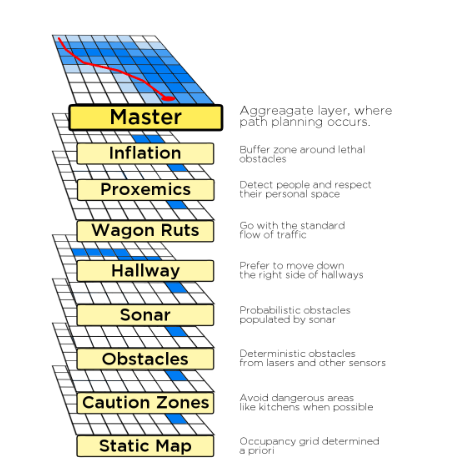
\includegraphics[width=0.6\textwidth]{mapa_camadas.png}\\
    }
    {\sourcecitation{\textcite{layered_costmaps}}}
\end{figure}

\subsection{Sensores e SLAM}

A escolha do sensor é importante para o mapeamento,
pois afeta a qualidade e quantidade de informações obtida pelo robô, além
de determinar a escolha das ferramentas utilizadas para o mapeamento do
ambiente~\cite{SensorAndSLAM}.

Sensores acústicos, como sonares e sensor de distância a laser, são utilizados
em ferramentas SLAM 2D tradicionais. Estes sistemas são robustos e bem estabelecidos,
com fácil integração ao sistema de navegação do ROS 2.

Porém, com o avanço da tecnologia, sensores RGB-D e câmeras estéreo estão se tornando
mais acessíveis, influenciando o desenvolvimento de sistemas de \textit{Visual} SLAM(VSLAM).
Dentre sistemas de VSLAM, destacam-se o ORB-SLAM3, OpenVSLAM e RTABMap, que possuem suporte
a câmeras RGB-D e permitem localização pura.
Em \textcite{VSLAM}, é feita uma comparação entre estes sistemas, mostrando que o
OpenVSLAM é a técnica mais adequada para maioria dos casos.
Porém, para ambientes internos com câmeras RGB-D, o RTABMap também teve um bom desempenho.
Estes sistemas, porém, não são integrados nativamente ao \textit{Navigation2}.

{ \color{red} deveria me aprofundar mais nos sistemas de slam? }
% CITAR~\cite{SLAMToolbox}

\section{Navigation2}

O \textit{Navigation2}(Nav2) é o sucessor do ROS \textit{navigation stack}, permitindo
a realização de tarefas complexas em diversos ambientes e classes de robôs cinemáticos.
Baseando-se no legado do \textit{navigation stack} do ROS 1, o Nav2 foi construído em cima
do ROS2, implementando técnicas mais modernas para ter um sistema modular propício para
ambientes dinâmicos com suporte a uma maior variedade de sensores~\cite{Nav2}.

\begin{figure}[htbp]
    {
        \centering
        \caption{Arquitetura do \textit{Navigation2}}.
        \label{fig:nav2_arc}
        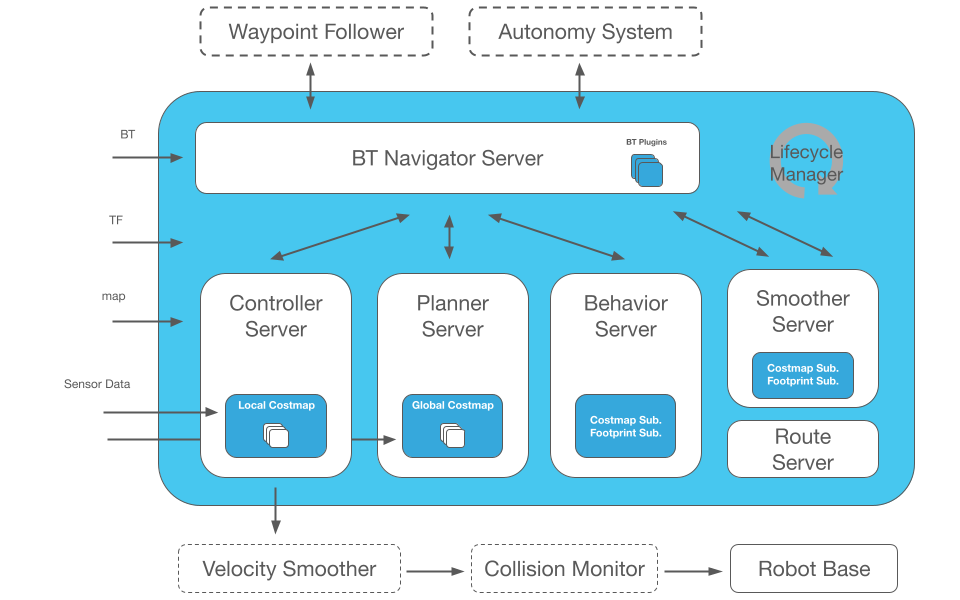
\includegraphics[width=0.9\textwidth]{nav2_architecture.png}\\
    }
    {\sourcecitation{\textcite{nav2_site}}}
\end{figure}

Na Figura \ref{fig:nav2_arc} é mostrada a arquitetura do Nav2.
O \textit{Behavior Tree(BT) Navigator Server} usa uma árvore de comportamento para
orquestrar as tarefas de navegação, ativando os servidores de controle, planejamento e
recuperação para navegar.
Para executar nós de \textit{actions}, normalmente são utilizados
\textit{Action servers} do ROS 2.
Esta árvore de comportamento pode ser configurada pelo usuário através de um arquivo
em XML, permitindo a descrição de comportamentos de navegação únicos sem
necessidade de programação.

Além disso, todos estes servidores utilizam o conceito de \textit{Managed Nodes},
também conhecidos como \textit{Lifecycle Nodes}.
Estes nós utilizam máquinas de estados para gerenciar seu ciclo de vida, utilizando
transições de estado desde sua criação a destruição.
No caso de falha ou desligamento, o nó vai do estado ativo ao estado finalizado seguindo
a máquina de estados, permitindo que o sistema seja finalizado de forma segura.

Na arquitetura também pode-se notar a utilização de dois mapas de custo, um local e
outro global.
O mapa local, utilizado no servidor do controlador, é utilizado para planejamento a curto
prazo e prevenção de colisão, enquanto o mapa global, utilizado no servidor de planejamento, é utilizado principalmente
para planejamento a longo prazo.

\chapter{Metodologia}
\label{desenvolvimento}

%O objetivo do robô Twil é, a partir de um ponto final, passado pelo rviz como uma mensagem
%--tipo da mensagem--, planejar uma trajetória até o destino, utilizando os dados
%dos sensores para ajustar o caminho evitando colisões.

%Para isso, o robô

\section{Descrição do robô}

falar do twil description
falar do plugin da camera
citar o pacote do intelrealsense
falar do controlador

\section{Configuração do Nav2}

\subsection{Ambiente de simulação}
\begin{figure}[htbp]
    {
        \centering
        \caption{Planta do 1º andar do prédio Centenário da EE-UFRGS}
        \label{fig:planta_centenario}
        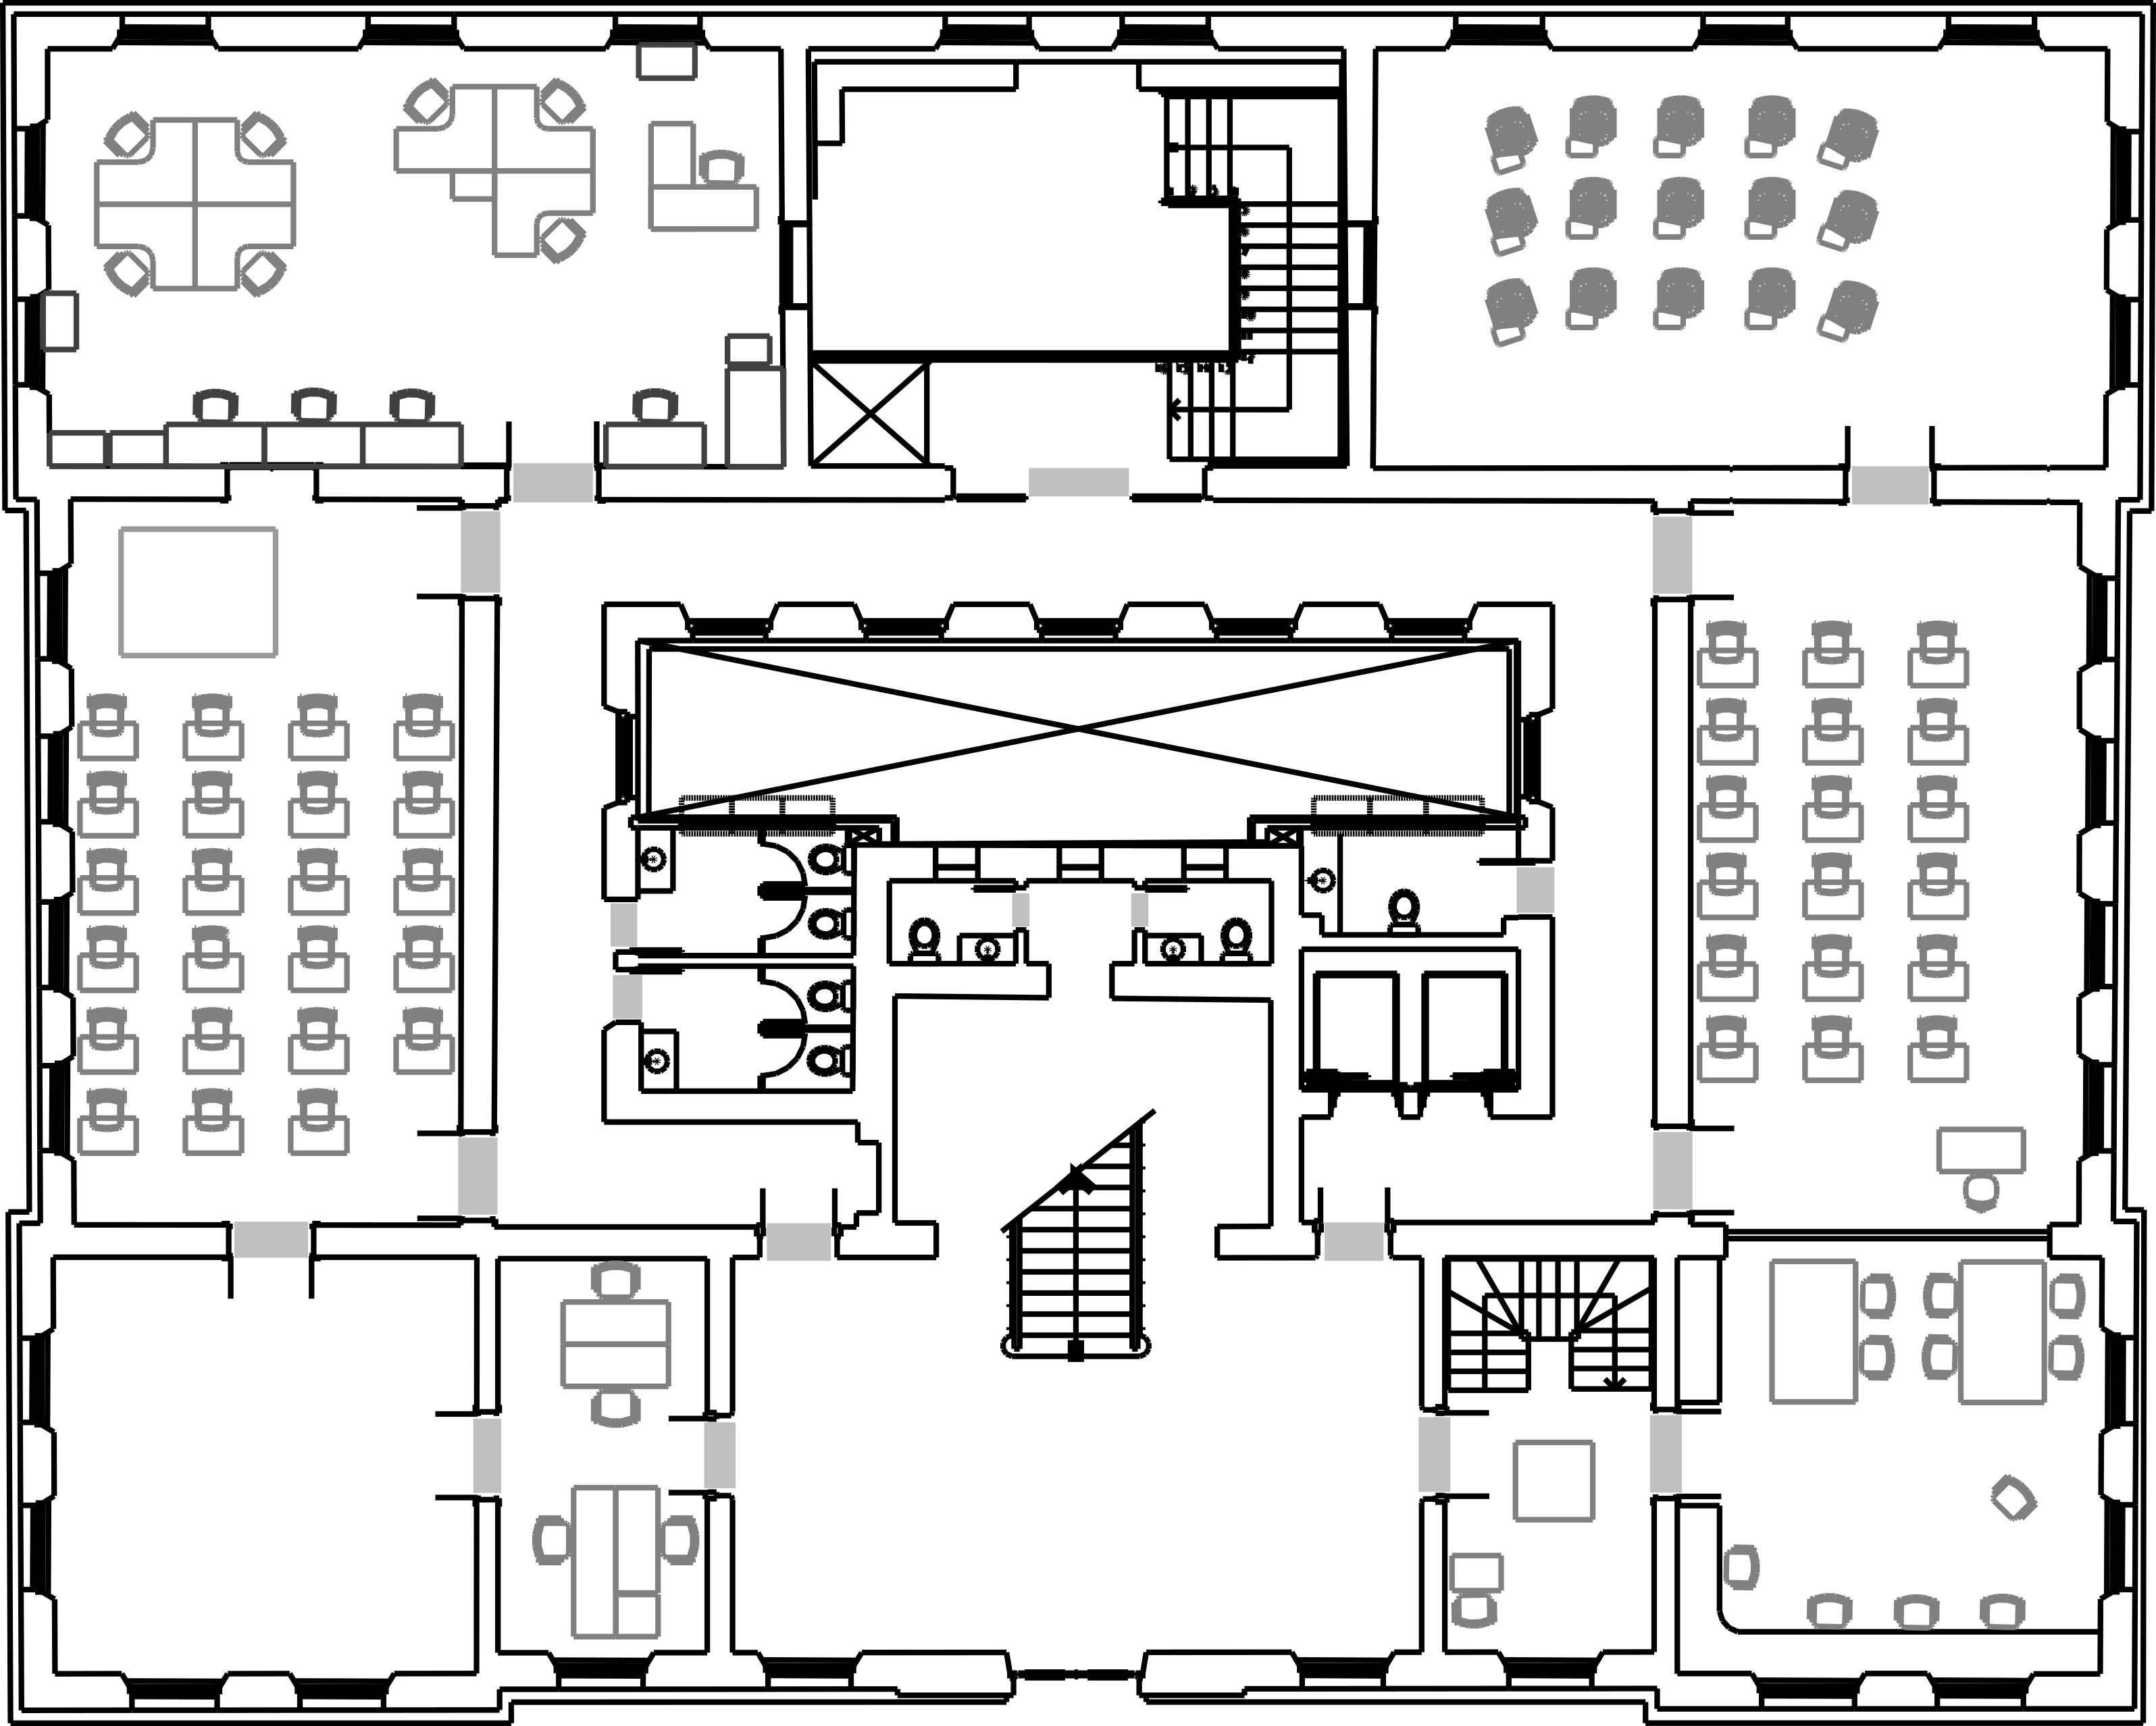
\includegraphics[width=0.5\textwidth]{centenario_floor_plan.png}\\
    }
    {\sourcecitation{citar o petry aqui}}
\end{figure}

\begin{figure}[htbp]
    {
        \centering
        \caption{Ambiente Gazebo com modelo do prédio Centenário da EE-UFRGS}
        \label{fig:gazebo_centenario}
        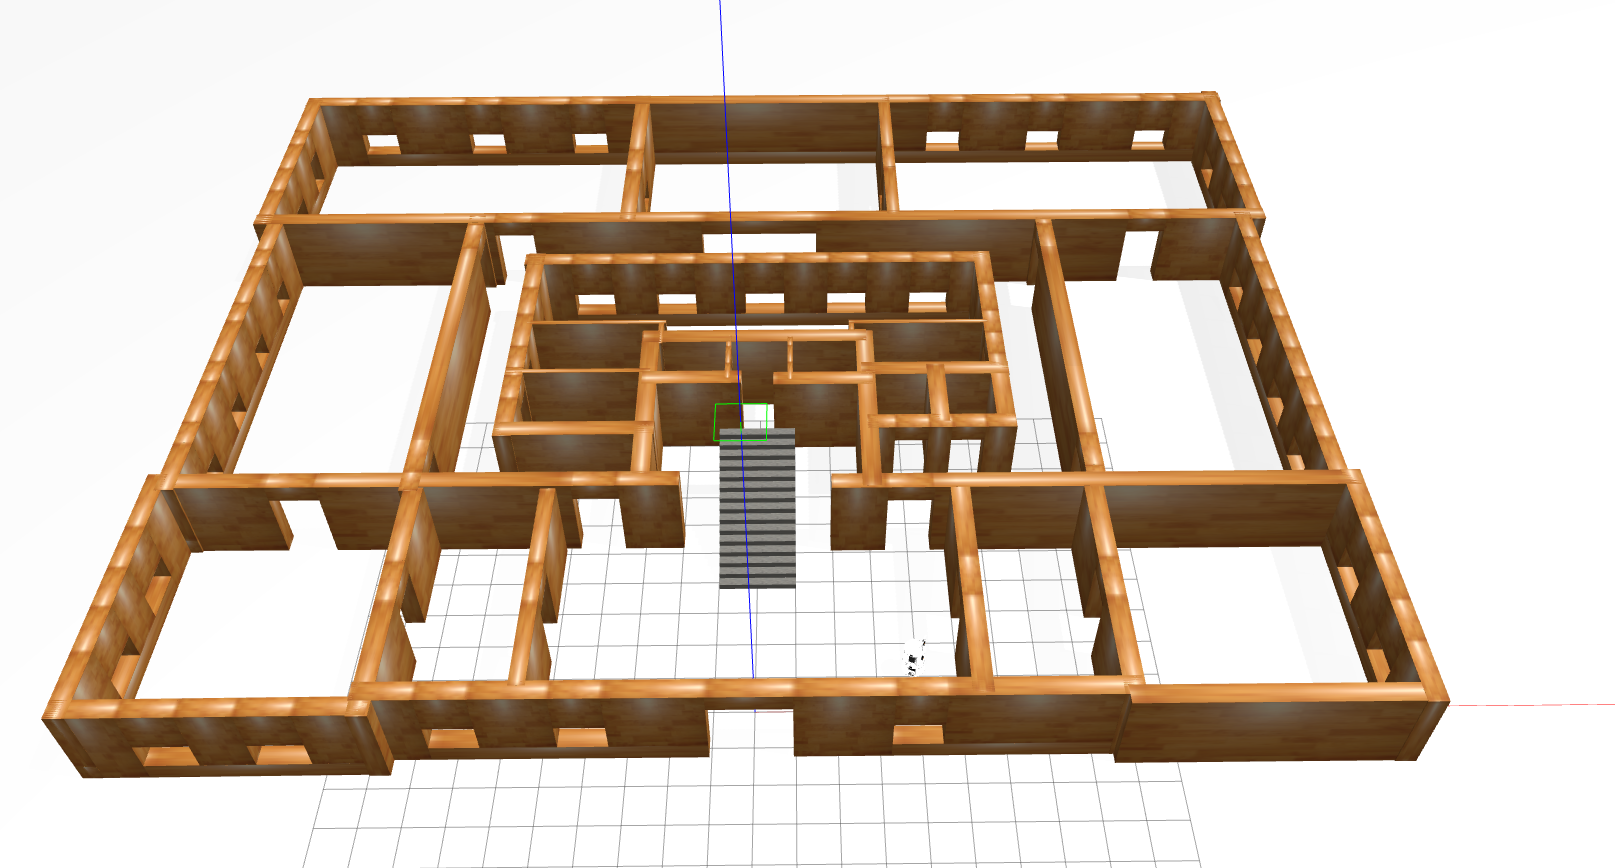
\includegraphics[width=0.8\textwidth]{gazebo.png}\\
    }
    {\sourcecitation{Autor}}
\end{figure}

\begin{figure}[htbp]
    {
        \centering
        \caption{RViz com robô twil no ambiente do prédio Centenário da EE-UFRGS}
        \label{fig:rviz_centenario}
        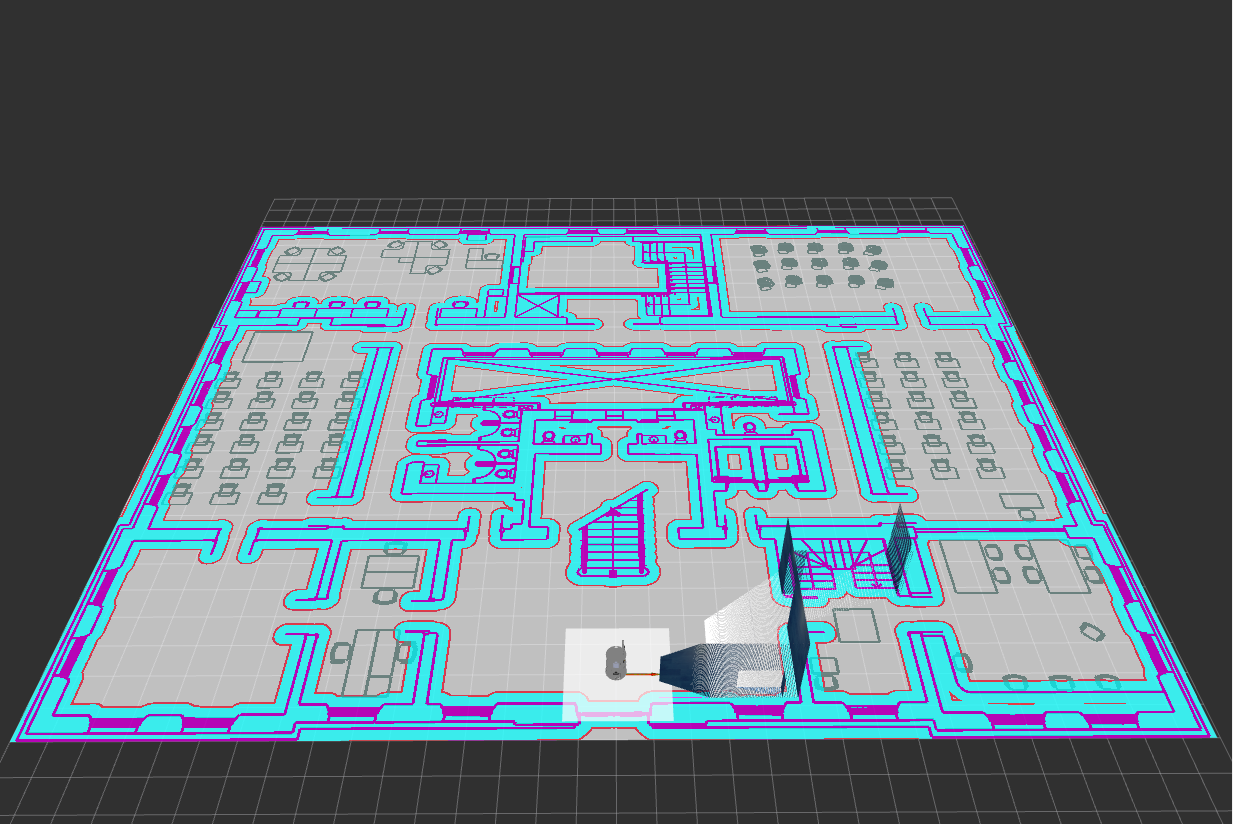
\includegraphics[width=0.8\textwidth]{rviz.png}\\
    }
    {\sourcecitation{Autor}}
\end{figure}

\subsection{Localização e Mapeamento}

\begin{figure}[htbp]
    {
        \centering
        \caption{RViz mostrando o erro de odometria \color{red}tirar essa?}
        \label{fig:erro_odom}
        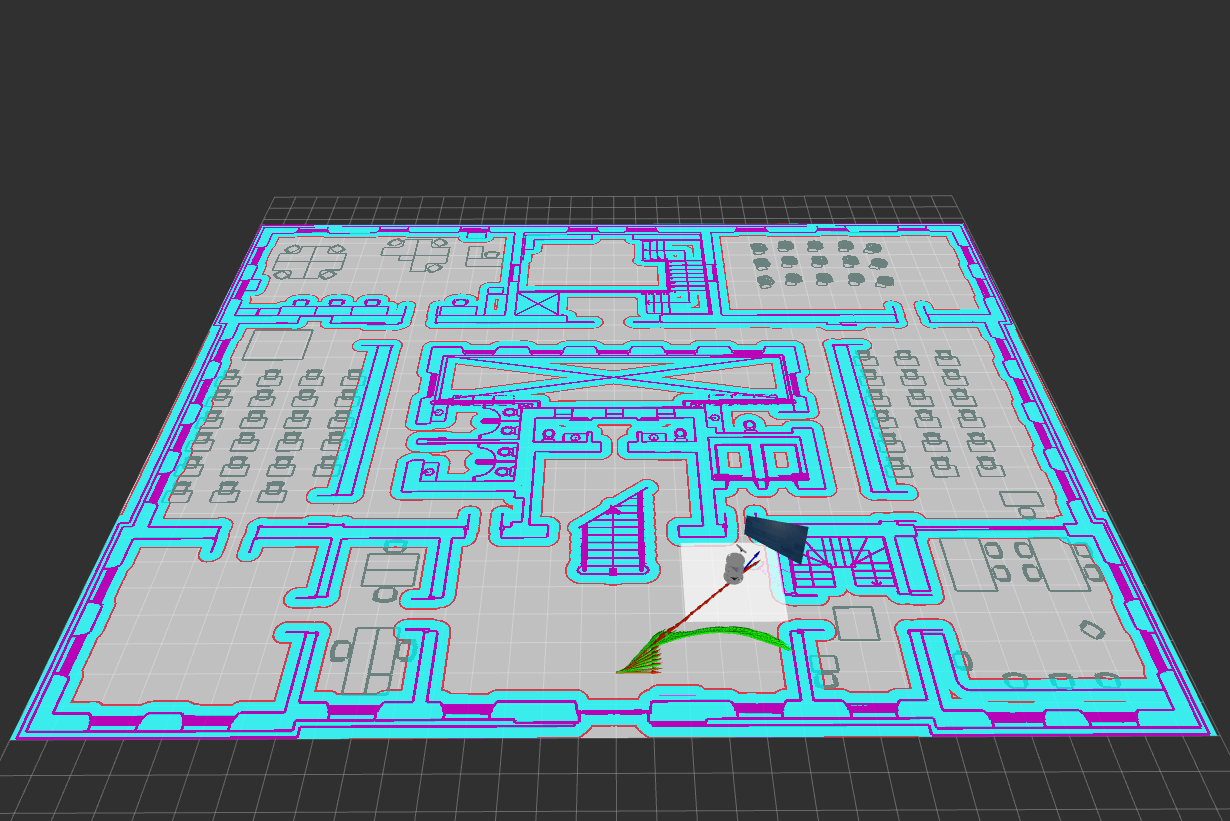
\includegraphics[width=0.5\textwidth]{erro_de_odometria.png}\\
    }
    {\sourcecitation{Autor}}
\end{figure}

\subsubsection{Mapas de custo}

Citar~\cite{ros_tuning_guide} para falar da inflation layer

nav2\_amcl e slam\_toolbox são slam 2d e só funcionam com mensagens do tipo LaserScan
(de sensores LIDAR, etc..)

para usar a câmera RGB-D na transformação map -> odom, teria que utilizar um pacote VSLAM


\chapter{Conclusão}
\label{conclusao}

falar do robô real
rosdeps/containerização


\printbibliography

\begin{appendix}

\end{appendix}


\begin{annex}
\end{annex}

\end{document}

